\chapter{Интегрирование функций}

\section{Определение первообразной}

\mcdfn{}{
    Пусть $ f(x) $ определена на $(a; b), a, b \in \ExtRset $

    Первообразной к функции $f(x)$ называется такая функция $F(x)$, определённая на $(a; b)$, что $ F'(x) = f(x) $
}

\mcex{}{
    Первообразной к $ \frac{1}{1 + x^2} $ будет $ \arctan(x) $

    Первообразной к $ \frac{1}{1 + x^2} $ будет $ \arctan(x) + 1 $

    Первообразной к $ \frac{1}{1 + x^2} $ будет $ \arctan(x) + \pi $
}

\section{Свойство первообразных}

\label{antiderivative_properties:2}

\mcthm{Свойство первообразных}{
    Пусть $ f(x) $ определена на $(a; b), a, b \in \ExtRset $

    Если $ F_1(x) $ и $ F_2(x) $ - первообразные к $f(x)$ на $(a; b)$, то

    $ F_1(x) - F_2(x) = const $

\mcprf{
\begin{split}
    & F_1(x) \text{ и } F_2(x) 
        \text{ дифференцируемы на } (a; b)
        \text{ и непрерывны на } [a; b] \\
    & \text{Тогда по теореме } \ref{theorem_corollary_2:1}: F_1(x) - F_2(x) = const \text{ на } [a; b] \\
\end{split}
}
}

\mcex{}{
    $ \int \frac{1}{x} dx = \ln | x | + C, C \in \Rset $, т.к.

    При $ x > 0: \ln'(x) = \frac{1}{x} $

    При $ x < 0: \ln'(-x) = \frac{1}{-x} \cdot (-1) = \frac{1}{x} $

    При этом, т.к. $ D_{\ln} = (-\infty; 0) \cup (0; +\infty) $, 
    то можно привести пример, когда предыдущая теорема не выполняется на $ D_{\ln} $:

    $ F_1(x) = \ln | x | $

    $ F_2(x) = \left\{ \begin{tabular}{l}
        $ \ln x, x > 0 $ \\
        $ \ln(-x) + 2, x < 0 $ \\
    \end{tabular} \right. $
}

\section{Неопределённый интеграл}

\subsection{Определение неопределённого интеграла}

\mcdfn{Неопределённый интеграл}{
    Неопределённым интегралом для $f(x)$ на $(a; b)$ называется множество первообразных $f(x)$

    Обозначение: $ \int f(x) dx = \{ F(x) + C \}_{C \in \Rset} $

    На практике пишут $ \int f(x) dx = F(x) + C $ и используют интеграл как функцию
}

\subsection{Свойства неопределённого интеграла}

\nt{
    Свойства неопределённого интеграла

\begin{tabular}{rl}
    $\bullet$ & $ \int 1 \cdot d F(x) = \int d F(x) = F(x) + C, C \in \Rset $ \\
    $\bullet$ & $ \left(\int f(x) dx\right)' = f(x) $ \\
              & $ d \left(\int f(x) dx\right) = f(x) dx $ \\
    $\bullet$ & $ \int f(x) + g(x) dx = \int f(x) dx + \int g(x) dx $ \\
\end{tabular}
}

\subsection{Теорема об интеграле сложной функции}

\mcthm{Теорема об интеграле сложной функции}{
    Если $F(x)$ - первообразная к $f(x)$ на $(a; b)$ и $ \phi(t) $ дифференцируема 
    на $(c; d) $, причём $ \phi((c; d)) \subseteq (a; b) $, то

    \[ \int f(\phi(t)) \phi'(t) dt = F(\phi(t)) + C, C \in \Rset \]

\mcprf{
\begin{split}
    & (F(\phi(t)))' = F'(\phi(t)) \phi'(t) = f(\phi(t)) \phi'(t) \\
\end{split}
}
}

\subsection{Формула подстановки}

\mcclm{Формула подстановки}{}{
    \[ \int f(\phi(t)) \phi'(t) dt = \int f(x) dx \vert_{x = \phi(t)} \]

    Проведём занесение функции под знак дифференциала:

    \[ \int f(\phi(t)) \phi'(t) dt = \int f(\phi(t)) d \phi(t) = \int f(x) dx \vert_{x = \phi(t)} \]
}

\mcex{}{
    \[ \int \sin x^2 dx^2 = -cos x^2 + C, C \Rset \]
}

\mcex{}{
    \[ \int x e^{\frac{-x^2}{2}} dx = 
        -\int e^{\frac{-x^2}{2}} d\left(\frac{-x^2}{2}\right) 
        = -e^{\frac{-x^2}{2}} + C, C \in \Rset \]
}

\subsection{Формула замены переменных}

\mcclm{Формула замены переменных}{}{
    \[ \int f(x) dx = \int f(\phi(t)) \phi'(t) dt \vert_{t = \phi^{-1}(x)} \text{, если $ \phi $ обратима} \]
}

\mcex{}{
    $ x \in (-1; 1) $:

    $ \int \sqrt[]{1 - x^2} dx
        = \left\vert x = \sin t, t \in (-\frac{\pi}{2}; \frac{\pi}{2}) \right\vert
        = \int \cos t d \sin t
        = \int \cos^2 t dt
        = \int \frac{\cos 2t + 1}{2} dt
        = \frac{1}{2} \left( \int \cos 2t dt + \int 1 dt \right)
        = \frac{1}{2} \left( \frac{1}{2} \sin 2t + t + C \right) 
        = \frac{1}{4} \sin 2t + \frac{1}{2} t + C
        = \frac{1}{4} \sin(2 \arcsin x) + \frac{1}{2} \arcsin x + C $
}

\subsection{Интегрирование по частям}

\mcthm{Формула интегрирования по частям}{
    $ f(x) $ и $ g(x) $ - дифференцируемы на $ (a; b) $

    $ \int f(x) d g(x) = f(x) g(x) - \int g(x) d f(x) $

\mcprf{
\begin{split}
    & d (f(x) g(x))
        = (f'(x) g(x) + f(x) g'(x)) dx
        = g(x) d f(x) + f(x) d g(x) \\
    & \int d (f(x) g(x)) = \int g(x) d f(x) + f(x) d g(x) \\
    & f(x) g(x) = \int (g(x) d f(x) + f(x) d g(x)) \\
    & f(x) g(x) - \int g(x) d f(x) = \int f(x) d g(x) \\
\end{split}
}
}

\mcex{}{
    $ \int x e^x dx = \int x d e^x = x e^x - \int e^x dx = x e^x - e^x + C, c \in \Rset $
}

\mcex{}{
    \[ \int \ln x dx = x \ln x - \int x d\ln x = x \ln x - \int 1 dx = x \ln x - x + C, C \in \Rset \]
}

\section{Определённый интеграл}

\subsection{Разбиение, диаметр разбиения, разметка разбиения}

\mcdfn{Разбиение отрезка}{
    Разбиением отрезка $[a; b]$ называется множество

    $ \tau = \{ [x_{i - 1}; x_i] \}_{i = 1}^{n} $,

    $ a = x_0 < x_1 < ... < x_n = b $
}

\mcex{Пример разбиения}{
    $[a; b] = [0; 2]$

    $ n = 5, \tau = \{ [0; 0.5], [0.5, 1], [1; 1.5], [1.5; 1.75], [1.75, 2] \} $

    $ a = 0 = x_0 < x_1 = 0.5 < x_2 = 1 < x_3 = 1.5 < x_4 = 1.75 < x_5 = 2 = b $
}

\mcdfn{Измельчение разбиения}{
    Пусть даны 2 разбиения:

    $ \tau = \{ [x_{i - 1}; x_i] \}_{i = 1}^{n} $

    $ \tau' = \{ [x'_{j - 1}; x'_j] \}_{j = 1}^{k} $

    $ \tau' $ является измельчением $ \tau $, если
    $ \forall i \, \exists j: x_i = x'_j $

    Обозначение: $ \tau' \succ \tau $ 
}

\nt{
    Если $ \tau' \succ \tau $, то $ k \ge n $, причём $ k = n \iff \tau' = \tau $
}

\mcex{Пример измельчения разбиения}{
    $ [a; b] = [0; 5]$

    $ n = 3, \tau = \{ [0; 1], [1; 3], [3; 5] \} $

    $ x_0 = 0, x_1 = 1, x_2 = 3, x_3 = 5 $

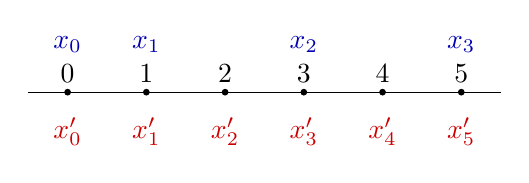
\begin{tikzpicture}
    \draw (0,0) -- (6,0);
    \filldraw[black] (0.5,0) circle (1pt) node[anchor=south]{0};
    \filldraw[black] (1.5,0) circle (1pt) node[anchor=south]{1};
    \filldraw[black] (2.5,0) circle (1pt) node[anchor=south]{2};
    \filldraw[black] (3.5,0) circle (1pt) node[anchor=south]{3};
    \filldraw[black] (4.5,0) circle (1pt) node[anchor=south]{4};
    \filldraw[black] (5.5,0) circle (1pt) node[anchor=south]{5};
    \filldraw[blue!70!black] (0.5,0.6) node[]{$x_{0}$};
    \filldraw[blue!70!black] (1.5,0.6) node[]{$x_{1}$};
    \filldraw[blue!70!black] (3.5,0.6) node[]{$x_{2}$};
    \filldraw[blue!70!black] (5.5,0.6) node[]{$x_{3}$};
    \filldraw[red!80!black] (0.5,-0.5) node[]{$x'_{0}$};
    \filldraw[red!80!black] (1.5,-0.5) node[]{$x'_{1}$};
    \filldraw[red!80!black] (2.5,-0.5) node[]{$x'_{2}$};
    \filldraw[red!80!black] (3.5,-0.5) node[]{$x'_{3}$};
    \filldraw[red!80!black] (4.5,-0.5) node[]{$x'_{4}$};
    \filldraw[red!80!black] (5.5,-0.5) node[]{$x'_{5}$};
\end{tikzpicture}

    $ k = 5, \tau' = \{ [0; 1], [1; 2], [2; 3], [3; 4], [4; 5] \} $

    $ x'_0 = 0, x'_1 = 1, x'_2 = 2, x'_3 = 3, x'_4 = 4, x'_5 = 5 $
}

\mcdfn{Диаметр разбиения}{
    Диаметр разбиения - это $ d(\tau) 
        = \underset{1 \le i \le n}{\max} (x_i - x_{i - 1}) 
        = \underset{1 \le i \le n}{\max} \Delta x_i $
}

\mcdfn{Разметка разбиения}{
    Разметка разбиения - это множество $ \{ \xi_i | \xi_i \in [x_{i - 1}; x_i] \}_{i = 1}^{n} $

    Разбиение, у которого есть разметка, называется размеченным разбиением
}

\subsection{Интегральная сумма Римана}

\mcdfn{Интегральная сумма Римана}{
    Интегральная сумма (Римана) - это \[ \sigma_{\tau}(f) = \sum_{i = 1}^{n} f(\xi_i) \Delta x_i \]
}

\subsection{Определение определённого интеграла по Коши}

\label{cauchy_integr_def:3}

\mcdfn{Определение определённого интеграла по Коши}{
    Число $I$ называется определённым интегралом $f(x)$ на $[a; b]$, если

    $ \forall \veps > 0 \,
        \exists \delta > 0 \,
        \forall \tau: d(\tau) < \delta \,
        \forall \text{ разметки } \{ \xi_i \}_{i = 1}^{n}: \,
        | \sigma_\tau(f) - I | < \veps $
}

\subsection{Определение определённого интеграла по Гейне}

\mcdfn{Определение определённого интеграла по Гейне}{
    Число $I$ называется определённым интегралом $f(x)$ на $[a; b]$, если

    $ \forall \text{ послед. } \tau_k: d(\tau_k) \underset{k \to +\infty}{\to} 0 \,
        \forall \{ \xi_{i}^{k} \}_{i = 1}^{n}: \,
        \sigma_{\tau_k}(f) \underset{k \to +\infty}{\to} I $
}

\subsection{Определение функции, интегрируемой по Риману}

\mcdfn{Определение интегрируемости по Риману}{
    Функция $f(x)$ интегрируема по Риману, если $\exists I \in \Rset[] $, т.ч.
    выполняется определение по Коши $\ref{cauchy_integr_def:3}$

    Обозначения: 

    $ f(x) \in R[a; b] $, где $R[a; b]$ - множество функций, интегрируемых по Риману на отрезке $[a; b]$

    $ I = \int_{a}^{b} f(x) dx $
}

\mcex{}{
    Пример функции, не интегрируемой по Риману:

    На отрезке $[0; 1]$ рассмотрим функцию Дирихле: 
    $ D(x) = \left\{ \begin{tabular}{l}
        $ 1, x \in \Qset $ \\
        $ 0, x \notin \Qset $ \\
    \end{tabular} \right. $

    Выберем первую разметку такую, что $ \forall i \in \{ 1, ..., n \}: \xi_i \in \Qset $

    Тогда $ \sigma_{\tau}(D) 
        = \sum_{i = 1}^{n} D(\xi_i) \Delta x_i 
        = \sum_{i = 1}^{n} \Delta x_i = b - a = 1 - 0 = 1 $

    Выберем вторую разметку такую, что $ \forall i \in \{ 1, ..., n \}: \xi_i \in \Rset \setminus \Qset $

    Тогда $ \sigma_{\tau}(D) 
        = \sum_{i = 1}^{n} D(\xi_i) \Delta x_i 
        = \sum_{i = 1}^{n} 0 \cdot \Delta x_i = 0 $
}

\subsection{Теорема об ограниченности функции, интегрируемой на отрезке}

\mcthm{Теорема об ограниченности функции, интегрируемой на отрезке}{
    Функция, $f(x)$ интегрируемая на $ [a; b] $, ограничена на $ [a; b] $

\mcprf{
\begin{split}
    & \text{1. Предположим от противного, т.е. функция не ограничена на отрезке} \\
    & \text{По определению интегрируемости для } \veps = 1: \\
    & \exists \delta > 0 \, 
        \forall \tau: d(\tau) < \delta \, 
        \forall \{ \xi_i \}_{i = 1}^{n}: \,
        | \sigma_\tau(f) - I | < 1\\
    & \text{Зафиксируем $\tau$. Хотя бы на 1 элементе $ \tau $ $f(x)$ не ограничена. БОО это первый отрезок $[x_0; x_1]$} \\
    & \text{Зафиксируем разметку везде кроме 1-ого отрезка: } \xi_2, \xi_2, ... \xi_n \\
    & | \sigma_\tau(f) | - | I | \le | \sigma_\tau(f) - I | \implies | \sigma_\tau(f) | < | I | + 1 \\
    & | f(\xi_1) | \Delta x_1 - \sum_{i = 2}^{n} | f(\xi_i) | \Delta x_i \le | \sigma_\tau(f) | 
        \implies | f(\xi_1) | \Delta x_1 < | I | + 1 + \sum_{i = 2}^{n} | f(\xi_i) | \Delta x_i \\
    & | f(\xi_1) | < \frac{| I | + 1 + \sum_{i = 2}^{n} | f(\xi_i) | \Delta x_i}{\Delta x_1} \\
    & \text{Обозначим } C = \frac{| I | + 1 + \sum_{i = 2}^{n} | f(\xi_i) | \Delta x_i}{\Delta x_1} > 0 \\
    & \text{Получили: } \forall \xi_1 \in [x_0; x_1]: | f(\xi_1) | < C \\
    & \text{Но на отрезке $[x_0; x_1]$ функция не ограничена } \implies \Contradiction \\
\end{split}
}
}

\subsection{Суммы Дарбу}

\subsubsection{Нижняя сумма Дарбу}

\mcdfn{Нижняя сумма Дарбу}{
    Пусть $ f(x) $ ограничена на $ [a; b] $, дано разбиение $ \tau $, 
    тогда нижней суммой Дарбу называется

    $ s_\tau = \sum_{i = 1}^{n} m_i \Delta x_i $, 
    где $ \forall i: m_i = \underset{x \in [x_{i - 1}; x_i]}{\inf} f(x) $
}

\subsubsection{Верхняя сумма Дарбу}

\mcdfn{Верхняя сумма Дарбу}{
    Пусть $ f(x) $ ограничена на $ [a; b] $, дано разбиение $ \tau $, 
    тогда верхней суммой Дарбу называется

    $ S_\tau = \sum_{i = 1}^{n} M_i \Delta x_i $, 
    где $ \forall i: M_i = \underset{x \in [x_{i - 1}; x_i]}{\sup} f(x) $
}

\subsubsection{Свойства сумм Дарбу}

\label{darboux_sums_props:4}

\mcclm{Свойства сумм Дарбу}{}{
\begin{tabular}{rl}
    $\bullet$ & $ s_\tau, S_\tau $ определены, если $ f(x) $ ограничена, 
                    т.е. $ s_\tau \in \Rset[] \wedge S_\tau \in \Rset[] $ \\
    $\bullet$ & Если $ \tau' \succ \tau $, то: \\
              & $ S_{\tau'} \le S_\tau $ \\
              & $ s_{\tau'} \ge s_\tau $ \\
    $\bullet$ & $ \forall \tau_1, \tau_2: s_{\tau_1} \le S_{\tau_2} $ \\
    $\bullet$ & $ s_\tau = \underset{ \{ \xi_i \}_{i = 1}^{n} }{\inf} \sigma_{\tau}(f) $ - инфинум по всем разметкам \\
              & $ S_\tau = \underset{ \{ \xi_i \}_{i = 1}^{n} }{\sup} \sigma_{\tau}(f) $ - супремум по всем разметкам \\
\end{tabular}

    Докажем 2-е свойство для нижних сумм Дарбу:
\mcprf{
\begin{split}
    & \text{Докажем для нижних сумм, для верхних сумм аналогично: } \\
    & s_\tau = \sum_{i = 1}^{n} m_i \Delta x_i \\
    & s_{\tau'} = \sum_{j = 1}^{k} m'_j \Delta x'_j \\
    & \forall i \, \exists n_{i - 1} < n_i: 
        \sum_{j = n_{i - 1} + 1}^{n_i} \Delta x'_j = \Delta x_i 
        \text{ и } 
        \cup_{j = n_{i - 1} + 1}^{n_i} [x'_{j - 1}; x'_j] = [x_{i - 1}; x_i] \\
    & 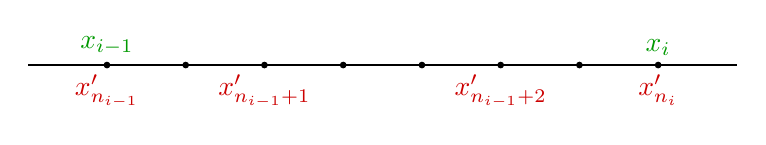
\begin{tikzpicture}
        \draw (0,0) -- (9,0);
        \filldraw[black] (1,0) circle (1pt);
        \filldraw[black] (2,0) circle (1pt);
        \filldraw[black] (3,0) circle (1pt);
        \filldraw[black] (4,0) circle (1pt);
        \filldraw[black] (5,0) circle (1pt);
        \filldraw[black] (6,0) circle (1pt);
        \filldraw[black] (7,0) circle (1pt);
        \filldraw[black] (8,0) circle (1pt);
        \filldraw[green!60!black] (1,0) node[anchor=south]{$x_{i-1}$};
        \filldraw[green!60!black] (8,0) node[anchor=south]{$x_{i}$};
        \filldraw[red!80!black] (1,0) node[anchor=north]{$x'_{n_{i - 1}}$};
        \filldraw[red!80!black] (3,0) node[anchor=north]{$x'_{n_{i - 1} + 1}$};
        \filldraw[red!80!black] (6,0) node[anchor=north]{$x'_{n_{i - 1} + 2}$};
        \filldraw[red!80!black] (8,0) node[anchor=north]{$x'_{n_i}$};
    \end{tikzpicture} \\
    & \text{Т.к. $m_i$ - $\inf f(x)$ на всём отрезке $[x_{i-1}; x_i]$, то } \forall j \in \{ n_{i - 1} + 1, ..., n_i \}: m'_j \ge m_i \\
    & \text{Тогда } m'_j \Delta x'_j \ge m_i \Delta x'_j \\
    & \text{Следовательно, } \sum_{j = n_{i - 1} + 1}^{n_i} m'_j \Delta x'_j 
        \ge \sum_{j = n_{i - 1} + 1}^{n_i} m_i \Delta x'_j 
        = m_i \Delta x_i \\
    & \text{Тогда } 
        \sum_{j = 1}^{k} m'_j \Delta x'_j \ge \sum_{i = 1}^{n} m_i \Delta x_i 
        \implies
        s_\tau' \ge s_\tau \\
\end{split}
}

    Докажем 3-е свойство:
\mcprf{
\begin{split}
    & \text{Рассмотрим разбиение $ \tau $, состоящее из точек $ \tau_1 $ и $ \tau_2 $, тогда }
        \tau \succ \tau_1, \tau_2 \\
    & \text{Следовательно, по 2-му свойству сумм Дарбу: } s_{\tau_1} \le s_{\tau} \le S_\tau \le S_{\tau_2} \\
\end{split}
}

    Докажем 4-е свойство:
\mcprf{
\begin{split}
    & s_\tau
        = \sum_{i = 1}^{n} \underset{\xi_i \in [x_{i - 1}; x_i]}{\inf f(\xi_i)} \Delta x_i 
        = \underset{ \{ \xi_i \}_{i = 1}^{n} }{\inf} \sum_{i = 1}^{n} f(\xi_i) \Delta x_i
        = \underset{ \{ \xi_i \}_{i = 1}^{n} }{\inf} \sigma_{\tau}(f) \\
\end{split}
}
}

\subsubsection{Интегралы Дарбу}

\mcdfn{Верхний интеграл Дарбу}{
    Верхним интегралом Дарбу называется $ I^* = \underset{\tau}{\inf} S_{\tau} $ - инфинум верхних сумм Дарбу по всем разбиениям
}

\mcdfn{Нижний интеграл Дарбу}{
    Нижним интегралом Дарбу называется $ I_* = \underset{\tau}{\sup} s_{\tau} $ - супремум нижних сумм Дарбу по всем разбиениям
}

\mcclarf{Уточнение}{
    $ s_\tau \le S_\tau \implies I_* \le I^* $
}

\subsection{Критерий Дарбу интегрируемости по Риману}

\mclemma{Лемма 1}{
    Пусть $ \tau' \succ \tau $ и у $ \tau' $ на p точек (т.е. границ отрезков) больше, чем у $\tau$

    Тогда $ 0 \le S_{\tau} - S_{\tau'} \le (M - m) \cdot p \cdot \delta $, 
        где $ \delta > d(\tau) $, 
            $ m = \underset{x \in [a; b]}{\inf} f(x) \in \Rset[] $,
            $ M = \underset{x \in [a; b]}{\sup} f(x) \in \Rset[] $
\mcproofpure{
\[
\begin{split}
    & \text{1. $S_{\tau} - S_{\tau'} \ge 0 $ по свойству 2 сумм Дарбу \ref{darboux_sums_props:4}} \\
    & \text{2. Рассмотрим случай, когда $p = 1$} \\
    & \text{ Пусть граница отрезка, которая есть в $\tau'$, но которой нет в $\tau$, имеет индекс $i$ } \\
    & 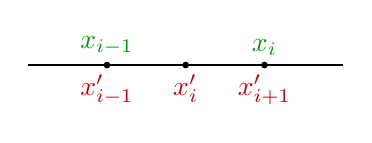
\begin{tikzpicture}
        \draw (0,0) -- (4,0);
        \filldraw[black] (1,0) circle (1pt);
        \filldraw[black] (2,0) circle (1pt);
        \filldraw[black] (3,0) circle (1pt);
        \filldraw[green!60!black] (1,0) node[anchor=south]{$x_{i-1}$};
        \filldraw[green!60!black] (3,0) node[anchor=south]{$x_{i}$};
        \filldraw[red!80!black] (1,0) node[anchor=north]{$x'_{i-1}$};
        \filldraw[red!80!black] (2,0) node[anchor=north]{$x'_{i}$};
        \filldraw[red!80!black] (3,0) node[anchor=north]{$x'_{i+1}$};
    \end{tikzpicture} \\
    & S_{\tau} = \sum_{j = 1}^{n} M_j \textcolor{green!60!black}{\Delta x_j} 
        \text{, где } M_j = \underset{x \in [\textcolor{green!60!black}{x_{j-1}}; \textcolor{green!60!black}{x_j}]}{\sup f(x)} \\
    & S_{\tau'} = \sum_{j = 1}^{n + 1} M'_j \textcolor{red!80!black}{\Delta x'_j}
        \text{, где } M'_j = \underset{x \in [\textcolor{red!80!black}{x'_{j-1}}; \textcolor{red!80!black}{x'_j}]}{\sup f(x)} \\
    & \text{Причём } 
        \forall j < i: \textcolor{green!60!black}{x_j} = \textcolor{red!80!black}{x'_j} \wedge M_j = M'_j 
        \text{ и } 
        \textcolor{green!60!black}{x_i} = \textcolor{red!80!black}{x'_{i+1}}
        \text{ и } 
        \forall j > i: \textcolor{green!60!black}{x_{j}} = \textcolor{red!80!black}{x'_{j + 1}} \wedge M_{j} = M'_{j + 1} \\
    & \text{Тогда } S_\tau - S_{\tau'} 
        = M_i \textcolor{green!60!black}{\Delta x_i} 
        - (M'_i \textcolor{red!80!black}{\Delta x'_i} + M'_{i + 1} \textcolor{red!80!black}{\Delta x'_{i + 1}}) 
        = M_i (\textcolor{red!80!black}{\Delta x'_i} + \textcolor{red!80!black}{\Delta x'_{i + 1}}) 
        - (M'_i \textcolor{red!80!black}{\Delta x'_i} + M'_{i + 1} \textcolor{red!80!black}{\Delta x'_{i + 1}})
        = \\
    &   = (M_i - M'_i) \textcolor{red!80!black}{\Delta x'_i} + (M_i - M'_{i+1}) \textcolor{red!80!black}{\Delta x'_{i + 1}}
        \le \left| \text{т.к. $M_i \le M$ и $M'_i \ge m$} \right|
        \le (M - m) \textcolor{red!80!black}{\Delta x'_i} + (M - m) \textcolor{red!80!black}{\Delta x'_{i + 1}} = \\
    &   = (M - m) \textcolor{green!60!black}{\Delta x_i} \le (M - m) \cdot d(\tau) < (M - m) \cdot \delta \\
\end{split}
\]

3. Для p > 1 доказывается итерационно, сводя для каждой из $p$ точек измельчения $\tau'$ к пункту 2.
}
}

\mclemma{Лемма Дарбу}{
    Пусть дан отрезок $[a; b]$ и функция $f(x)$, непрерывная на отрезке $[a; b]$, тогда

    \[ I^* = \lim_{d \to 0} S_{\tau} \]

    Это означает, что $ \forall \veps > 0 \, \exists \delta > 0 \, \forall \tau: d(\tau) < \delta: | S_\tau - I^* | < \veps $
\mcprf{
\begin{split}
    & \text{1. Если $m = M$, то функция - константа на отрезке $[a; b]$, тогда все верхние суммы равны} \\
    & \text{$ f(a) \cdot (b - a) \implies I^* = f(a) \cdot (b - a)$, т.к. $I^*$ - это инфинум верхних сумм по всем разбиениям} \\
    & \text{2. Иначе, если $m \ne M$, то $m < M$} \\
    & \text{Пусть дано $\veps > 0$, тогда} \\
    & I^* = \underset{\tau}{\inf S_\tau} \implies \exists \tau^*: \left| S_{\tau^*} - I^* \right| < \frac{\veps}{2} \\
    & \text{$I^*$ - инфинум всех верхних сумм } \implies S_{\tau^*} \ge I^* \implies S_{\tau^*} - I^* < \frac{\veps}{2} \\
    & \text{Пусть в $\tau^*$ p точек (границ отрезков внутри $(a; b)$), т.е. $\tau^*$ состоит из $p+1$ отрезка } \\
    & \text{Положим } \delta = \frac{\veps}{2 (M - n) p} \\
    & \text{Построено $\delta$, тогда пусть дано разбиение $\tau$ т.ч. $d(\tau) < \delta$} \\
    & \text{Составим разбиение $\tau'$ из границ отрезков разбиений $\tau$ и $\tau^*$, тогда $ \tau' \succ \tau \wedge \tau' \succ \tau^* $,}\\
    & \text{и при этом в $\tau'$ не более чем на $p$ больше точек (границ отрезков), чем в $\tau$, тогда по Лемме 1} \\
    & 0 \le S_\tau - S_{\tau'} \le (M - m) \cdot p \cdot \delta = \frac{\veps}{2} \\
    & \text{(если в $\tau'$ меньше, чем на p больше точек, чем в $\tau$, то неравенство также выполняется)} \\
    & \text{$\tau'$ - измельчение $\tau^*$ по построению } \implies S_{\tau'} \le S_{\tau^*} \\
    & \text{$I^*$ - инфинум всех верхних сумм } \implies S_{\tau'} \ge I^* \implies I^* \le S_{\tau'} \le S_{\tau^*} \\
    & S_{\tau^*} - I^* < \frac{\veps}{2} \implies S_{\tau'} - I^* < \frac{\veps}{2} \\
    & \left. \begin{tabular}{l}
        $ 0 \le S_\tau - S_{\tau'} < \frac{\veps}{2} $ \\
        $ 0 \le S_{\tau'} - I^* < \frac{\veps}{2} $ \\
    \end{tabular} \right\} \implies 0 \le S_\tau - I^* < \veps \implies \left| S_\tau - I^* \right| < \veps \\
\end{split}
}
}

\nt{
    Аналогичная лемма верна и для случая нижних сумм: \[ I_* = \lim_{d \to 0} s_{\tau} \]
}

\mcthm{Критерий Дарбу интегрируемости по Риману}{
    Ограниченная функция $ f(x) $ интегрируема на $ [a; b] \iff I^* = I_* $

    Используя введённые обозначения, $f(x) \in R[a; b] \iff f(x) \text{ ограничена и } I^* = I_*  $

\mcprf{
\begin{split}
    & "\implies" \\
    & \text{Предположим от противного, т.е. функция интегрируема и } I_* \ne I^* \implies I_* < I^* \\
    & \text{По определению интегрируемости:} \\
    & \forall \veps > 0 \, 
        \exists \delta > 0 \, 
        \forall \tau: d(\tau) < \delta 
        \forall \{ \xi_i \}_{i = 1}^{n}: \,
        | \sigma_\tau(f) - I | < \veps \\ 
    & | \sigma_\tau(f) - I | < \veps 
        \implies I - \veps < \sigma_\tau(f) < I + \veps 
        \implies I - \veps \le s_\tau \le S_\tau \le I + \veps \text{ по сво-ву 4} \\
    & s_\tau \le I_* < I^* \le S_\tau \implies S_\tau - s_\tau \ge I^* - I_* > 0
        \text{, но при этом } \forall \veps > 0: S_\tau - s_\tau \le 2 \veps 
        \implies \Contradiction \\
    & "\impliedby" \\
    & \text{Обозначим $I = I_* = I^*$ и покажем, что выполняется определение, т.е.}  \\
    & \forall \veps > 0 \, \exists \delta > 0 \, \forall \tau: d(\tau) < \delta \, \forall \{ \xi_i \}_{i = 1}^{n}: | \sigma_\tau(f) - I | < \veps \\
    & | \sigma_\tau(f) - I | < \veps \implies I - \veps < \sigma_\tau(f) < I + \veps \\
    & \text{По определению сумм Дарбу } s_\tau \le \sigma_\tau(f) \le S_\tau \\
    & \text{По лемме Дарбу $ \exists \delta_1 > d(\tau):  S_\tau < I^* + \veps $} \\
    & \text{аналогично $ \exists \delta_2 > d(\tau): s_\tau > I_* - \veps $} \\
    & \text{Положим $\delta = \min(\delta_1, \delta_2)$, тогда: } 
        I_* - \veps 
        < \sigma_\tau(f) 
        < I^* + \veps \implies I - \veps 
        < \sigma_\tau(f) 
        < I^* + \veps 
        = I + \veps \\
\end{split}
}
}

\subsection{Определение равномерной непрерывности}

\mcdfn{Определение равномерной непрерывности}
{
    Функция $f(x)$ называется равномерно непрерывной на $E \subseteq \Rset[] $, если

    $ \forall \veps > 0 \, \exists \delta = \delta(\veps) > 0 \, \forall x_1, x_2 \in E: | x_1 - x_2 | < \delta \implies | f(x_1) - f(x_2) | < \veps $
}

\nt{
    $f(x)$ равномерно непрерывна на $E \implies f(x)$ непрерывна на $E$, но обратное, вообще говоря, не верно
}

\mcex{Пример к замечанию}{
    $ E = (0; 1), f(x) = \frac{1}{x} $

    $f(x)$ непрерывна на $E$, покажем, что равномерной непрерывности нет:

    Рассмотрим последовательность аргументов: $x_n = \frac{1}{n}$, тогда $x_{n+1} - x_n \underset{n \to +\infty}{\to} 0 $,

    но при этом $f(x_{n+1}) - f(x_n) = 1$

    Положим $\veps = 0.5$, тогда т.к. $x_{n+1} - x_n \underset{n \to +\infty}{\to} 0 $, то можно выбрать $x_i$ и $x_j$, т.ч. $|x_i - x_j| < \delta(0.5)$,
    но при этом $ |f(x_1) - f(x_2)| = 1 > 0.5 = \veps $
}

\subsection{Теорема Кантора}

\mcthm{Теорема Кантора (для случая функции на отрезке)}{
    Если $f(x)$ непрерывна на $[a; b]$, то $f(x)$ равномерно непрерывна на $[a; b]$
\mcprf{
\begin{split}
    & \text{Предположим от противного, тогда в отрицании определения выберем конкретные значения $\delta$:} \\
    & \exists \veps_0 \, \forall \delta = \frac{1}{n} \, \exists x'_n, x_n'' \in [a; b]: | x'_n - x''_n | < \frac{1}{n}: \left| f\left(x'_n\right) - f\left(x''_n\right) \right| > \veps_0 \\
    & \text{Ч.п. $\{ x'_n \}$ и $\{ x''_n \}$ ограничены $\implies$ по теореме Больцано-Вейерштрасса из них можно } \\
    & \text{выделить сходящиеся подпоследовательности: } \exists x'_{n_k} \underset{k \to +\infty}{\to} x_0 \in [a; b] \\
    & \text{При этом по теореме о зажатой последовательности } x''_{n_k} \underset{k \to +\infty}{\to} x_0 \\
    & \text{$f(x)$ непрерывна в точке $x_0$, тогда по определению непрерывности в точке по Гейне:} \\
    & f\left(x'_{n_k}\right) \underset{k \to +\infty}{\to} f(x_0) \\
    & f\left(x''_{n_k}\right) \underset{k \to +\infty}{\to} f(x_0) \\
    & \text{Но по предположению } \left| f\left(x'_n\right) - f\left(x''_n\right) \right| > \veps_0 \implies \Contradiction \\
\end{split}
}
}

\subsection{Теорема об интегрируемости непрерывной функции}

\mcthm{Теорема об интегрируемости непрерывной функции}{
    Если $f(x)$ непрерывна на $[a; b]$, то $f(x) \in R[a; b]$

\mcprf{
\begin{split}
    & 1. f(x) \text{ непрерывна на } [a; b] \implies \text{ по теореме Кантора $f(x)$ равномерно непрерывна на } \\
    & [a; b] \text{, тогда по определению: } 
        \forall \veps > 0 \, 
        \exists \delta > 0 \, 
        \forall x_1, x_2 \in [a; b]: 
        | x_1 - x_2 | < \delta \implies | f(x_1) - f(x_2) | < \veps \\
    & \text{2. Для любого $\veps > 0$ рассмотрим разбиение $\tau$ отрезка $[a; b]$ с диаметром $d(\tau) < \delta$, тогда} \\
    &   0 \le I^* - I_* 
        \le S_\tau - s_\tau 
        = \sum_{i = 1}^{n} \left(M_i - m_i\right) \Delta x_i
        = \sum_{i = 1}^{n} \left(f(\xi_i) - f(\eta_i)\right) \Delta x_i \text{, т.к. $f$ непрерывна на $[a; b]$} \\
    & \forall i: | \xi_i - \eta_i | \le d(\tau) < \delta \implies |f(\xi_i) - f(\eta_i)| < \veps \implies 0 \ge f(\xi_i) - f(\eta_i) < \veps \\
    & \text{Тогда } 
        \sum_{i = 1}^{n} \left(f(\xi_i) - f(\eta_i)\right) \Delta x_i  \le \sum_{i = 1}^{n} \veps \Delta x_i = \veps \cdot (b - a) \\
    & \text{$I^* - I_*$ - неотрицательное число, и при этом } \forall \veps > 0: I^* - I_* < \veps (b - a) \implies I^* - I_* = 0 \\
\end{split}
}
}

\subsection{Теорема об интегрируемости монотонной функции}

\mcthm{Теорема об интегрируемости монотонной функции}{
    Если $f(x)$ определена и монотонна на $[a; b]$, то $f(x) \in R[a; b]$
\mcprf{
\begin{split}
    & \text{БОО докажем для неубывающей функции} \\
    & \text{1. Для любого $\delta > 0$ рассмотрим разбиение $\tau$ отрезка $[a; b]$ с диаметром $d(\tau) < \delta$, тогда} \\
    & 0 \le I^* - I_* 
        \le S_\tau - s_\tau 
        = \sum_{i = 1}^{n} \left(M_i - m_i\right) \Delta x_i
        = \sum_{i = 1}^{n} \left(f(x_i) - f(x_{i-1})\right) \Delta x_i
        < \sum_{i = 1}^{n} \left(f(x_i) - f(x_{i-1})\right) \delta 
        = \\
    &   = \delta \sum_{i = 1}^{n} \left(f(x_i) - f(x_{i-1})\right) 
        = \delta \left(f(b) - f(a)\right) \\
    & \text{$I^* - I_*$ - неотрицательное число, и при этом } \forall \delta > 0: I^* - I_* < \delta \left(f(b) - f(a)\right) \implies I^* - I_* = 0 \\
\end{split}
}
}

\subsection{Элементы теории меры}

\subsubsection{Критерий Лебега интегрируемости по Риману}

\mcthm{Критерий Лебега интегрируемости по Риману (без док-ва)}{
    Функция $f(x) \in R[a; b] \iff $ функция $f(x)$ ограничена и множество точек разрыва функции - множество меры ноль по Лебегу
}

\subsubsection{Определение множества меры ноль по Лебегу}

\mcdfn{Определение множества меры ноль по Лебегу}{
    Множество $E \subseteq \Rset[] $ называется множеством нулевой меры Лебега, если

    $ \forall \veps > 0 \, \exists \text{ не более чем счётный набор интервалов } \{ (a_i; b_i) \}_{i = 1}^{+\infty} $, такой что

    1. $ E \subseteq \cup_{i = 1}^{+\infty} (a_i; b_i) $, т.е. объединение всех интервалов покрывает множество $E$

    2. $ \sum_{i = 1}^{+\infty} b_i - a_i \le \veps $

    Обозначение: $ \mu(E) = 0 $
}

\mcex{Пример множества меры ноль по Лебегу}{
    Покажем, что $ \Qset[] \subseteq \Rset[] $ - множество нулевой меры Лебега
\mcprf{
\begin{split}
    & \text{1. } \Qset[] \cong \Nset[] \implies \Qset[] = \{ q_i \}_{i = 1}^{+\infty} \\    
    & \text{2. } \forall i \in \Nset[]: (a_i; b_i) = U_\frac{\veps}{2^{i+1}}(q_i) \implies \Qset[] \subseteq \cup_{i = 1}^{+\infty} (a_i; b_i) \\
    & \text{3. При этом } \sum_{i = 1}^{+\infty} b_i - a_i = \sum_{i = 1}^{+\infty} 2 \cdot \frac{\veps}{2^{i+1}} = \veps \le \veps \\
\end{split}
}
}

\subsubsection{Свойства множеств меры ноль по Лебегу}

\mcthm{Свойства множеств меры ноль по Лебегу}{
\begin{tabular}{rl}
    1. & Если $A \subseteq \Rset[]$ нулевой меры Лебега и 
        $B \subseteq A$, то $B$ тоже множество нулевой меры Лебега \\
       & (это свойство меры называется полнотой) \\
    2. & Если множества $X, Y$ - нулевой меры Лебега, то $X \cup Y$ - нулевой меры Лебега \\
\end{tabular}

Докажем 1-е свойство:
\mcprf{
\begin{split}
    & \text{$\forall \veps > 0$ по определению множества меры ноль по Лебегу построим покрытие} \\
    & \text{ множества $A: \{ (a_i; b_i) \}_{i=1}^{+\infty} $, т.ч. $\sum_{i = 1}^{+\infty} b_i - a_i \le \veps$} \\
    & \text{$B \subseteq A \implies B \subseteq \cup_{i = 1}^{+\infty} (a_i; b_i)$} \\
\end{split}
}

Докажем 2-е свойство:
\mcprf{
\begin{split}
    & \text{Пусть дано $\veps > 0$, тогда:} \\
    & \text{Для $\frac{\veps}{2}$ по определению множества нулевой меры Лебега построим покрытия } \\
    & \text{для множеств $X$ и $Y$: } \{(a_i; b_i)\}_{i = 1}^{+\infty} \text{ и } \{(c_i; d_i)\}_{i = 1}^{+\infty} \text{ соответственно} \\
    & \text{Тогда для множества $X \cup Y$ построим покрытие } \{(e_i; f_i)\}_{i = 1}^{+\infty} \text{ такое что} \\
    & e_i = \left\{ \begin{tabular}{l}
        $ a_j, i = 2 j $ \\
        $ c_j, i = 2 j + 1 $ \\
    \end{tabular} \right. \\
    & f_i = \left\{ \begin{tabular}{l}
        $ b_j, i = 2 j $ \\
        $ d_j, i = 2 j + 1 $ \\
    \end{tabular} \right. \\
    & \text{Тогда $ X \cup Y \subseteq \cup_{i=1}^{+\infty} (e_i; f_i) $ и: } \\
    & \sum_{i=1}^{+\infty} \left| f_i - e_i \right|
    = \sum_{j=1}^{+\infty} | b_j - a_j | + \sum_{j=1}^{+\infty} | d_j - c_j |
    \le \frac{\veps}{2} + \frac{\veps}{2}
    = \veps \\
\end{split}
}
}

\nt{
    Из 1 и 2 свойств следует, что разность, пересечение и 
    симметрическая разность множеств нулевой меры Лебега -
    также множества нулевой меры Лебега
}

\subsection{Свойства определённого интеграла}

\mcthmBreakable{Свойства определённого интеграла}{
\begin{tabular}{rl}
    1.  & Линейность: \\
        & Пусть $ f, g \in R[a; b] $, тогда \\
        & $
        \forall \alpha, \beta \in \Rset[]: \alpha f + \beta g \in R[a; b] 
        \wedge \int_{a}^{b} \left( \alpha f(x) + \beta g(x) \right) dx 
        = \alpha \int_{a}^{b} f(x) dx + \beta \int_{a}^{b} g(x) dx 
        $\\
    2.  & Если $f, g \in R[a; b]$, то $ f \cdot g \in R[a; b] \wedge | f | \in R[a; b] $ \\
        & (здесь $f \cdot g$ - это произведение, а не композиция, т.е. $\forall x \in \Rset: (f \cdot g)(x) = f(x) \cdot g(x) $) \\
    3.  & Аддетивность: если $f \in R[a; c]$, и $b \in [a; c]$ 
        то: \\
        & $f \in R[a; b] \cup R[b; c] $ и 
            $ \int_{a}^{c} f(x) dx 
            = \int_{a}^{b} f(x) dx 
            + \int_{b}^{c} f(x) dx $ \\
    4.  & Интегрируемось неравенств: 
            $f, g \in R[a; b]$ и 
            $ \forall x \in [a; b]: f(x) \le g(x) $, то:\\
        & $ \int_{a}^{b} f(x) dx \le \int_{a}^{b} g(x) dx $ \\ 
    5.  & Теорема о среднем: \\
        & Если $f(x)$ непрерывна на $[a; b]$, то
            $ \exists \xi \in [a; b]: 
            f(\xi) = \frac{1}{b - a} \int_{a}^{b} f(x) dx $ \\
    6.  & Оценка интеграла: \\
        & Если $f(x) \in R[a; b]$, то: \\
        & $ \left| \int_{a}^{b} f(x) dx \right| 
            \le \int_{a}^{b} \left| f(x) \right| dx $  \\
\end{tabular}

Докажем 1-е свойство:
\mcprf{
\begin{split}
    & \text{1. По критерию Лебега интегрируемости по Риману: $ f, g $ - ограниченные на $[a;b]$ функции и} \\
    & X_f \text{ - множество точек разрыва функции $f$ и при этом $\mu(X_f) = 0$} \\
    & X_g \text{ - множество точек разрыва функции $g$ и при этом $\mu(X_g) = 0$} \\
    & \text{Пусть $ X_{\alpha f + \beta g} $ - множество точек разрыва непрерывной на $[a;b]$ функции $\alpha f + \beta g$} \\
    & X_{\alpha f + \beta g} \subseteq X_f \cup X_g \implies \mu(X_{\alpha f + \beta g}) = 0 \\
    & \text{Тогда по критерию Лебега интегрируемости по Риману $ \alpha f + \beta g \in R[a; b] $} \\
    & \text{2. Рассмотрим последовательность разбиений $\tau_k$:} 
        \forall \tau_k
        \forall \{ \xi_i \}_{i=1}^{+\infty} 
        \sigma_{\tau}(\alpha f + \beta g) 
            = \alpha \sigma_{\tau}(f) + \beta \sigma_{\tau}(g) \text{, т.к.} \\
    &   \sigma_{\tau}(\alpha f + \beta g)
        = \sum_{i=1}^{n} \left( \alpha f(\xi_i) + \beta g(\xi_i) \right) \cdot \Delta x_i
        = \sum_{i=1}^{n} \alpha f(\xi_i) \cdot \Delta x_i + \sum_{i=1}^{n} \beta g(\xi_i) \cdot \Delta x_i 
        = \alpha \sigma_{\tau}(f) + \beta \sigma_{\tau}(g) \\
    & \text{По определению Гейне интегрируемости по Риману:} \\
    & \sigma_{\tau}(\alpha f + \beta g) \underset{k \to +\infty}{\to} 
        \int_{a}^{b} \left(\alpha f(x) + \beta g(x)\right) dx \\
    & \alpha \sigma_{\tau}(f) \underset{k \to +\infty}{\to} 
        \alpha \int_{a}^{b} f(x) dx \\
    & \beta \sigma_{\tau}(g) \underset{k \to +\infty}{\to} 
        \beta \int_{a}^{b} g(x) dx \\
    & \implies \int_{a}^{b} \left(\alpha f(x) + \beta g(x)\right) dx 
        = \alpha \int_{a}^{b} f(x) dx + \beta \int_{a}^{b} g(x) dx \\
\end{split}
}

2-е свойство:
\begin{equation*}
\begin{split}
    & \text{2-е свойство доказывается аналогично 1-ому доказательству, т.к. множества точек разрыва } \\
    & \text{функций $f \cdot g$ и $|f|$ - множества меры ноль по Лебегу и эти функции непрерывны на $[a; b]$ } \\
    & \text{ } \\
\end{split}
\end{equation*}

Докажем 3-е свойство:
\mcprf{
\begin{split}
    & \text{1. $f \in R[a; c] \implies$ и на отрезках $[a; b]$ и $[b; c]$ 
        она непрерывна и её множества точек разрыва } \\
    & \text{ на этих отрезках тоже множества меры ноль по Лебегу } 
            \implies f \in R[a; b] \wedge f \in R[b; c] \\
    & \text{2. По определению интегрируемости по Гейне: } \\
    & \forall \tau_k \text{ разбиения отрезка $[a;c]$ т.ч. }
        d(\tau_k) \underset{k \to +\infty}{\to} 0 \,
        \forall \{ \xi_i^k \}_{i=1}^{n}:
        \sigma_{\tau_k}(f) 
        = \sum_{i=1}^{n} f(\xi_i^k)\Delta x^k 
        \underset{k \to +\infty}{\to} 
        \int_{a}^{c} f(x) dx \\
    & \text{Будем рассматривать последовательность $ \tau_k^0 $,
        такую что точка $b$ является точкой данного} \\
    & \text{разбиения, т.е. является границей одного из отрезков } \\
    & \text{(вообще говоря, если $a < b < c$, то 2-ых отрезков) } \\
    & \text{Тогда } \tau_k^0 = \tau_k^1 \cup \tau_k^2 \text{, 
    где $\tau_k^1$ - разбиение $[a; b]$, 
        $\tau_k^2$ - разбиение $[b; c]$ } \\
    & \text{Следовательно, } 
        \sigma_{\tau_k^0}(f) 
      = \sigma_{\tau_k^1}(f)
      + \sigma_{\tau_k^2}(f) \\
    & \text{По 1 пункту и интегрируемости по Гейне:} \\
    & \sigma_{\tau_k^1}(f) \underset{k \to +\infty}{\to} \int_{a}^{b} f(x) dx \\
    & \sigma_{\tau_k^2}(f) \underset{k \to +\infty}{\to} \int_{b}^{c} f(x) dx \\
    & \text{Тогда }     
        \int_{a}^{c} f(x) dx 
        = \int_{a}^{b} f(x) dx 
        + \int_{b}^{c} f(x) dx \\
\end{split}
}

Докажем 4-е свойство:
\mcprf{
\begin{split}
    & \text{Рассмотрим $ h(x) = g(x) - f(x) \in R[a; b] $. 
        $\forall x \in [a; b]: h(x) \ge 0$ } \\
    & \text{Тогда } 
        \forall \tau: \sigma_{\tau}(f) \ge 0
        \implies \int_{a}^{b} h(x) dx \ge 0
        \implies \int_{a}^{b} g(x) dx - \int_{a}^{b} f(x) dx \ge 0 
        \implies \int_{a}^{b} g(x) dx 
            \ge \int_{a}^{b} f(x) dx \\
\end{split}
}

Докажем 5-е свойство (формально, теорему о среднем для интегралов)

\mcprf{
\begin{split}
    & \text{1. т.к. $f$ непрерывна на $[a; b]$, то } 
        \forall x \in [a; b]: m \le f(x) \le M 
    \text{, где } 
        m = \underset{x \in [a; b]}{\inf} f(x) \in \Rset[]
    \text{ и }
        M = \underset{x \in [a; b]}{\sup} f(x) \in \Rset[] \\
    & \text{2. По 4-ому свойству определённых интегралов: } \\
    & \int_{a}^{b} m \, dx
        \le \int_{a}^{b} f(x) dx
        \le \int_{a}^{b} M \, dx \\
    & m (b - a)
    \le \int_{a}^{b} f(x) dx
    \le M (b - a) \\
    & m \le \frac{1}{b - a} \int_{a}^{b} f(x) dx 
        \le M \\
    & \text{ $f$ - непрерывная функция на $[a; b]$ } 
        \implies E_f = [m; M] 
        \implies \exists \xi \in [a; b]: 
        f(\xi) = \frac{1}{b - a} \int_{a}^{b} f(x) dx \\
\end{split}
}

Докажем 6-е свойство:
\mcprf{
\begin{split}
    & \text{1. } \forall x \in [a; b]: 
        -\left|f(x)\right| \le f(x) \le \left|f(x)\right| \\
    & f \in R[a; b] \implies 
        \int_{a}^{b} -\left|f(x)\right| dx
        \le \int_{a}^{b} f(x) dx 
        \le \int_{a}^{b} \left|f(x)\right| dx 
        \implies \\
    & \implies 
        - \int_{a}^{b} \left|f(x)\right| dx
        \le \int_{a}^{b} f(x) dx 
        \le \int_{a}^{b} \left|f(x)\right| dx 
        \implies
        \left| \int_{a}^{b} f(x) dx \right| 
        \le \int_{a}^{b} \left|f(x)\right| dx \\
\end{split}
}
}

\section{Обобщённое понятие интеграла}

\mcclm{Обобщённое понятие интеграла}{}{
    $ \forall a, b \in \Rset[] $ (если $f \in R[\min(a; b); \max(a; b)]$) доопределим:

    \[ \int_{a}^{a} f(x) dx = 0 \]

    \[ \int_{b}^{a} f(x) dx = - \int_{a}^{b} f(x) dx \]
}

\nt{
    $ \forall c_1, c_2, c_3 \in [a; b]: $
    \[
        \int_{c_1}^{c_3} f(x) dx
        = \int_{c_1}^{c_2} f(x) dx
        + \int_{c_2}^{c_3} f(x) dx
    \]
}

\nt{
    Уточним оценку интеграла (6-е свойство):

    \[
        \forall c_1, c_2 \in [a; b]:
        \left| \int_{c_1}^{c_2} f(x) dx \right| 
        \le \left| \int_{c_1}^{c_2} \left| f(x) \right| dx \right|
    \]
}

\subsection{Интеграл с переменным верхним пределом}

\mcdfn{Интеграл с переменным верхним пределом}{
    Пусть $f \in R[\alpha; \beta] $ и $ a, x \in [\alpha; \beta] $, тогда введём функцию $F$, т.ч.:

    \[ F(x) = \int_{a}^{x} f(t) dt \]

    Заметим, что $F(a) = 0$
}

\subsection{Теорема 1 об интеграле с переменным верхним пределом}

\mcthm{Теорема 1 об интеграле с переменным верхним пределом}{
    $F(x)$ непрерывна на $[\alpha; \beta]$
\mcprf{
\begin{split}
    & \text{1. Обозначим } M = \left| \underset{x \in [\alpha; \beta]}{\sup f(x)} \right| \in \Rset[] \\
    & \text{Тогда } \forall x \in [\alpha; \beta]: f(x) \le | f(x) | \le M \\
    & \text{2. } \left| F(x + \Delta x) - F(x) \right|
        = \left| \int_{a}^{x + \Delta x} f(t) dt 
          - \int_{a}^{x} f(t) dt  \right|
        = \left| \int_{x}^{x + \Delta x} f(t) dt \right|
        \le \left| \int_{x}^{x + \Delta x} \left|f(t)\right| dt \right| \le \\
    &   \le \left| \int_{x}^{x + \Delta x} M dt \right|
        = \left| M \Delta x \right| 
        = M \left| \Delta x \right| \\
    & \left( -M \Delta x \le F(x + \Delta x) - F(x) \le M \Delta x \right)
        \wedge \left( M \Delta x \underset{\Delta x \to 0}{\to} 0 \right)
        \implies  F(x + \Delta x) - F(x) \underset{\Delta x \to 0}{\to} 0 \\
    & \text{Тогда } 
        \lim_{\Delta x \to 0} \left(F(x + \Delta x) - F(x)\right) = 0 
        \implies \lim_{\Delta x \to 0} F(x + \Delta x) = F(x) \\
\end{split}
}
}

\subsection{Теорема 2 об интеграле с переменным верхним пределом}

\mcthm{Теорема 2 об интеграле с переменным верхним пределом}{
    $f(x) \in R[a; b] $ и непрерывна на $[\alpha; \beta]$, то
    $F(x)$ дифференцируема на $(\alpha; \beta)$ и $F'(x) = f(x)$
\mcprf{
\begin{split}
    & \frac{F(x + \Delta x) - F(x)}{\Delta x} 
        = \frac{1}{\Delta x} \int_{x}^{x + \Delta x} f(t) dt = \\
    &   = \left|\text{по теореме о среднем $\exists \xi = \xi(\Delta x) \in [\min(x; x+\Delta x); \max(x; x+\Delta x)]$}\right|
        = f(\xi) \underset{\Delta x \to 0}{\to} f(x) \\
    & \text{То есть по определению производной } 
        \forall x \in [\alpha; \beta]: F'(x) = f(x) \\
\end{split}
}
}

\subsection{Формула Ньютона-Лейбница}

\mcclm{Формула Ньютона-Лейбница}{}{
    Если $\Phi(x) $ - первообразная функции $f(x)$ на $(\alpha; \beta)$ и 
    $f(x)$ непрерывна на $[\alpha; \beta]$, то $\forall a, b \in [\alpha; \beta]$:
    \[ \int_{a}^{b} f(x) dx = \Phi(b) - \Phi(a) \]
\mcprf{
\begin{split}
    & F(b) = \int_{a}^{b} f(x) dx = F(b) \\
    & \text{$F(x)$ - первообразная функции $f(x)$ на $(\alpha; \beta) 
        \implies 
            \exists C \in \Rset[] \, 
            \forall x \in (\alpha; \beta): 
            F(x) = \Phi(x) + C $} \\
    & F(a) = \Phi(a) + C \wedge F(a) = 0 \implies C = - \Phi(a) 
        \implies F(b) = \Phi(b) + C = \Phi(b) - \Phi(a) \\
\end{split}    
}
}
